\documentclass{article}
\usepackage{graphicx} % Required for inserting images
\usepackage{blindtext}
\usepackage{titlesec}
\usepackage{listings}
\usepackage{xcolor}
\usepackage[left=2.5cm,right=2.5cm,top=2.5cm,bottom=2.5cm]{geometry}
\usepackage{multicol}
\usepackage[dvipsnames]{xcolor}
\usepackage{amsmath}
\usepackage{newtxtext}
\usepackage{changepage}
\setlength{\columnsep}{0.75cm}
\usepackage{biblatex}
\addbibresource{references.bib}
\usepackage{lipsum}
\newcommand*\rfrac[2]{{}^{#1}\!/_{#2}}
\usepackage{caption}
\usepackage{enumerate}
\captionsetup[figure]{font=footnotesize}
\definecolor{MSBlue}{rgb}{.204,.353,.541}
\definecolor{MSLightBlue}{rgb}{.31,.506,.741}

\lstset{
    basicstyle=\ttfamily\small, % 코드 폰트 크기
    backgroundcolor=\color{gray!10}, % 배경색 설정
    keywordstyle=\color{blue}, % 키워드 색상
    commentstyle=\color{green}, % 주석 색상
    stringstyle=\color{red}, % 문자열 색상
    numbers=left, % 왼쪽에 줄 번호 추가
    numberstyle=\tiny\color{gray}, % 줄 번호 스타일
    stepnumber=1, % 모든 줄에 번호 추가
    frame=single, % 테두리 추가
    breaklines=true, % 줄 바꿈
    tabsize=4, % 탭 크기
    showspaces=false, % 공백 표시 비활성화
    showstringspaces=false % 문자열의 공백 표시 비활성화
}

\usepackage{tcolorbox} % For creating color boxes
\newtcolorbox{mybox}[1]{colback=MSLightBlue!18!white,colframe=MSBlue,fonttitle=\sffamily\bfseries,title=#1}

\usepackage{fancyhdr}
\pagestyle{fancy}
\fancyhf{}
\rhead{20 September 2024}
\lhead{}
\chead{\textbf{Problem Set 2}}
\fancyfoot[C]{\thepage}
\fancyfoot[R]{}

% Set formats for each heading level
\titleformat*{\section}{\large\bfseries\sffamily\color{MSBlue}}
\titleformat*{\subsection}{\normalsize\bfseries\sffamily\color{MSLightBlue}}
\titleformat*{\subsubsection}{\itshape}

\newenvironment{Figure}
  {\par\medskip\noindent\minipage{\linewidth}}
  {\endminipage\par\medskip}

\makeatletter
\renewcommand{\maketitle}{\bgroup\setlength{\parindent}{0pt}
\begin{flushleft}
  \textbf{\@title}

  \@author
\end{flushleft}\egroup
}
\makeatother

\title{\LARGE {\fontfamily{qhv}\selectfont \textcolor{MSBlue}{Problem Set 2}}}

\author{
\small{\textit{\textsuperscript{1}}}}

\date{August 2023}

\begin{document}

\maketitle

\begin{mybox}{Question 1}
Let the initial wavefunction
\[
\Psi(x, t = 0) = \frac{1}{\sqrt{2}}(\phi_1(x) - \phi_3(x))
\]
where $\phi_i(x)$ is the $i^{th}$ lowest-energy eigenstate of the particle in a box.
\begin{itemize}
    \item[(a)] Give the analytic expression for the probability density.
    \item[(b)] Give the analytic expression for the expected evolution of the probability density.
    \item[(c)] Explain how the expected evolution of the probability density relates to the expected result for a nonstationary state.
    \item[(d)] Give the analytic expression for the average position as a function of time.
\end{itemize}
\end{mybox}

\begin{adjustwidth}{5pt}{5pt}

\subsection*{Part A}
At time t=0, the probability density is given by:
\begin{align*}
  |\Psi(x, t = 0)|^2 &= \left| \frac{1}{\sqrt{2}} (\phi_1(x) - \phi_3(x)) \right|^2 \\
  &= \frac{1}{2} \left[ |\phi_1(x)|^2 + |\phi_3(x)|^2 - \phi_1^*(x) \phi_3(x) - \phi_3^*(x) \phi_1(x) \right] \\
  &= \frac{1}{2} \left[ |\phi_1(x)|^2 + |\phi_3(x)|^2 - 2 \, \text{Re}[\phi_1^*(x) \phi_3(x)] \right]
\end{align*}

\noindent For the particle in a box with length $L$, the orthonormal eigenstates are:
\[
\phi_n(x) = \sqrt{\frac{2}{L}} \sin \left( \frac{n \pi x}{L} \right), \quad n = 1, 2, 3, \dots
\]

\noindent Substituting $\phi_1(x) = \sqrt{\frac{2}{L}} \sin \left( \frac{\pi x}{L} \right)$ and $\phi_3(x) = \sqrt{\frac{2}{L}} \sin \left( \frac{3 \pi x}{L} \right)$, we get:
\begin{align*}
  |\Psi(x, t = 0)|^2 &= \frac{1}{2} \left[ \frac{2}{L} \sin^2 \left( \frac{\pi x}{L} \right) + \frac{2}{L} \sin^2 \left( \frac{3 \pi x}{L} \right) - 2 \frac{2}{L} \sin \left( \frac{\pi x}{L} \right) \sin \left( \frac{3 \pi x}{L} \right) \right] \\
  &= \frac{1}{L} \left[ \sin^2 \left( \frac{\pi x}{L} \right) + \sin^2 \left( \frac{3 \pi x}{L} \right) - 2 \sin \left( \frac{\pi x}{L} \right) \sin \left( \frac{3 \pi x}{L} \right) \right], \quad \text{(the last term is the interference term)}.
\end{align*}

\subsection*{Part B}
At time $t$, the wave function is given by:
\[
\phi_n(x, t) = e^{-iE_n t/\hbar}~\phi_n(x,t=0)
= e^{-iE_n t/\hbar}~\phi_n(x)
\]
\begin{equation}
\Psi(x, t) = \frac{1}{\sqrt{2}} \left( \phi_1(x,t) - \phi_3(x,t) \right)
=
\frac{1}{\sqrt{2}} \left( \phi_1(x) e^{-iE_1 t/\hbar} - \phi_3(x) e^{-iE_3 t/\hbar} \right)
\end{equation}
where $E_n = n^2 \pi^2 \hbar^2 / 2 M L$ and M is a mass of the particle.\\
Then, the probability density is:
\begin{align*}
  |\Psi(x, t)|^2 &= \left| \frac{1}{\sqrt{2}} \left( \phi_1(x) e^{-iE_1 t/\hbar} - \phi_3(x) e^{-iE_3 t/\hbar} \right) \right|^2 \\
  &= \frac{1}{2} \left[ |\phi_1(x)|^2 + |\phi_3(x)|^2 - 2 \text{Re}[\phi_1^*(x) \phi_3(x) e^{-i(E_3 - E_1) t/\hbar}] \right] \\
  &= \frac{1}{L} \left[ \sin^2 \left( \frac{\pi x}{L} \right) + \sin^2 \left( \frac{3 \pi x}{L} \right) - 2 \sin \left( \frac{\pi x}{L} \right) \sin \left( \frac{3 \pi x}{L} \right) \cos \left( \frac{(E_3 - E_1) t}{\hbar} \right) \right]\\
  &=\frac{1}{L} \left[ \sin^2 \left( \frac{\pi x}{L} \right) + \sin^2 \left( \frac{3 \pi x}{L} \right) - 2 \sin \left( \frac{\pi x}{L} \right) \sin \left( \frac{3 \pi x}{L} \right) \cos \left( \frac{4 \pi^2 \hbar t}{ML^2} \right) \right] \\
\end{align*}

\subsection*{Part C}

\noindent The evolution of the probability density will evolve periodically as time progresses per the $\cos\left(\frac{(E_{3} - E_{1})t}{\hbar}\right)$ term. Since the nonstationary wavefunction is a linear combination of two orthonormal eigenstates, the expectation value of an observable will look as such: $\langle \hat{A} \rangle = \langle \Psi(x,t) \mid \hat{A} \mid \Psi(x,t) \rangle
$. Where $\Psi(x,t)$ can be linearly expanded out using formula (1) from Part B.\\ 
For a nonstationary state, the time dependent nature of the expectation value of $\hat{A}$ is not always guaranteed. For example, Hermitian Operators of the form $ \hat{A} | \phi_{n}\rangle = \lambda_{n} | \phi_{n} \rangle$, which means that $\hat{A}$ have a simultaneous eigenbasis with $\hat{H}$ ~($[\hat{A},\hat{H}]=0$), will have an expectation value of the form: $\langle \hat{A} \rangle = \sum_{m} \lambda_{m}P(\lambda_{m}) = \sum_{m} \lambda_{m}|\langle\phi_{m}|\Psi(x)\rangle |^2 $, where the dependancy to time no longer exists. While for the probability density of a particle in a box, there will be a dependancy with respect to time. \\
If $\hat{A}=\hat{x}$, then we have to consider another approach since $\phi_i$ are energy (momentum) eigenstates but not position eigenstates. We can think about the case that the expectation value of the $\hat{A}$ degenerate for $| 
\phi_i \rangle$ and $| 
\phi_j \rangle$ (don't need to be eigenstates of $\hat{A}$), $\langle \phi_i | \hat{A}|\phi_i\rangle = \langle \phi_j | \hat{A}|\phi_j\rangle = \lambda$. Then, the expectation value of $\hat{A}$ for any superposition of $| 
\phi_i \rangle$ and $| 
\phi_j \rangle$ will be time-independent, as $\langle \hat{A} \rangle = \lambda~\alpha(t) + \lambda~(1-\alpha(t)) = \lambda$. This results can be generalized to the case of multiple states with degenerate expectation value (we can observe this at (b)-vii).


\subsection*{Part D}
The average position $\langle x(t) \rangle$ is given by:
\[
\langle x(t) \rangle = \int_0^L x |\Psi(x, t)|^2 \, dx
\]
Substituting the expression for $\Psi(x, t)$:
\[
\langle x(t) \rangle = \frac{1}{2} \int_0^L x \left( |\phi_1(x)|^2 + |\phi_3(x)|^2 - 2 \text{Re}[\phi_1^*(x) \phi_3(x) e^{-i(E_3 - E_1) t/\hbar}] \right) dx
\]

\noindent Since $\phi_1(x) = \sqrt{\frac{2}{L}} \sin\left(\frac{\pi x}{L}\right)$ and $\phi_3(x) = \sqrt{\frac{2}{L}} \sin\left(\frac{3\pi x}{L}\right)$ are symmetric about the center of the box ($x = L/2$), their individual contributions to the integral are constant when calculating the time-dependent shift:
\[
\int_0^L x |\phi_1(x)|^2 \, dx = \int_0^L x |\phi_3(x)|^2 \, dx = \frac{L}{2}
\]

\noindent The time dependence in $\langle x(t) \rangle$ arises from the cross term:
$-2 \text{Re} \left[ \phi_1^*(x) \phi_3(x) e^{-i(E_3 - E_1)t/\hbar} \right] = -2 \phi_1(x) \phi_3(x) \cos\left( \frac{(E_3 - E_1) t}{\hbar} \right)$

\noindent The average position can now be expressed as:
\[
\begin{aligned}
\langle x(t) \rangle &= \frac{L}{2} + A \cos\left( \frac{(E_3 - E_1) t}{\hbar} \right)
&= \frac{L}{2} + A \cos\left( \frac{4 \pi^2 \hbar t}{M L^2} \right)
\end{aligned}\]
where
\[
\begin{aligned}
A &= -\int_0^L x \phi_1(x) \phi_3(x) \, dx \\
&= -\int_0^L x \left( \sqrt{\frac{2}{L}} \sin\left(\frac{\pi x}{L}\right) \right) \left( \sqrt{\frac{2}{L}} \sin\left(\frac{3\pi x}{L}\right) \right) \, dx \\
&= -\frac{2}{L} \int_0^L x \sin\left(\frac{\pi x}{L}\right) \sin\left(\frac{3\pi x}{L}\right) \, dx \\
&= -\frac{1}{L} \int_0^L x \left[ \cos\left(\frac{2\pi x}{L}\right) - \cos\left(\frac{4\pi x}{L}\right) \right] \, dx \\
&= 0
\end{aligned}
\]

\noindent This indicates that while the probability density oscillates in time, which is the oscillation between $\phi_1$ and $\phi_3$ states, the particle's average position do not oscillate in time. This is because the particle's average positions corresponding to each $\phi_1$ and $\phi_3$ states coincides with each other.
\end{adjustwidth}

\begin{mybox}{Question 2}
Let the initial wavefunction be defined as the Gaussian wavepacket
\[
\Psi(x, t = 0) = \mathcal{N} e^{-a^2(x-L/2)^2/2}
\]
where $\mathcal{N}$ is the normalization coefficient, $L = 5 \, \textup{\AA}$, and $a = 4 \, \textup{\AA}^{-1}$.
\begin{itemize}
    \item[(a)] Demonstrate analytically whether $\Psi(x, t = 0)$ is a stationary state for a particle-in-a-box potential.
    \item[(b)] Using the accompanying Jupyter notebook:
    \begin{enumerate}[i.]
        \item Explain what the function $f(N) = \sum_{i=1}^N c_i^{*}c_i$ represents.
        \item Plot $f(N)$ for the given expansion coefficients $c_i$.
        \item Calculate $\mathrm{lim}_{N\rightarrow\infty} f(N).$
        \item Explain what $f(N)$ says about the number of expansion terms required to accurately simulate the wavefunction.
        \item Plot $|\Psi(x,t)|^2$ at several choices of $t$ to show how the wavefunction changes in time.
        \item Explain what $|\Psi(x,t)|^2$ tells us about the motion of a particle in a box.
        \item Plot $\langle x(t) \rangle$ and $\langle (x-L/2)^2(t) \rangle$.
        \item Explain the significance of $\langle x(t) \rangle$ and $\langle (x-L/2)^2(t) \rangle$ and their relationships.
    \end{enumerate}
\end{itemize}
\end{mybox}

\begin{adjustwidth}{5pt}{5pt}

\subsection*{Part A}
 A stationary state is an eigenfunction of the Hamiltonian $H$ of the system.

 $\bar{H} \Psi = E \Psi$ , start with time independent Schrodinger Equation.

 For Particle in a Box, $V(x) = 0$
\[
\frac{-i\hbar^2}{2m} \frac{\partial^2}{\partial x^2} \mathcal{N} e^{-a^2 \left(x - \frac{L}{2}\right)^2 / 2} = E \text{  }\mathcal{N} e^{-a^2 \left(x - \frac{L}{2}\right)^2 / 2}
\]

Take the first derivative:
\[
\frac{\partial}{\partial x}\mathcal{N} e^{-a^2 \left(x - \frac{L}{2}\right)^2 / 2} = \mathcal{N} e^{-a^2 \left(x - \frac{L}{2}\right)^2 / 2} * (-\alpha^2(x- \frac{L}{2}))
\]

Take the second derivative:
\[
\frac{\partial^2}{\partial x^2}\mathcal{N} e^{-a^2 \left(x - \frac{L}{2}\right)^2 / 2} * (-\alpha^2(x- \frac{L}{2})) = -\alpha^2\mathcal{N} e^{-a^2 \left(x - \frac{L}{2}\right)^2 / 2} + \mathcal{N} e^{-a^2 \left(x - \frac{L}{2}\right)^2 / 2}(-\alpha^2(x-\frac{L}{2}))^2
\]

Re-substitute the partial into the original Schrodinger Equation and simplify by representing the wavefunction as $\Psi(x, t = 0) = \mathcal{N} e^{-a^2(x-L/2)^2/2}$

\[
\frac{-i\hbar^2}{2m} \left( -\alpha^2 \Psi(x) + \Psi(x) \left(-\alpha^2 (x - \frac{L}{2})\right)^2 \right) = E \Psi(x)
\]
Factor out a $\Psi(x)$ from the left hand side and divide both sides by $\Psi(x)$.

\[
\frac{-i\hbar^2}{2m} \left( -\alpha^2  + \left(-\alpha^2 (x - \frac{L}{2})\right)^2 \right) \neq E 
\]
Since there is still a $x$ dependency in the l.h.s. (E is not well-defined), we know that $\Psi(x)$ is not an eigenfunction of the Hamiltonian operator, and therefore it is not a stationary state for a particle-in-a-box potential.
\subsection*{Part B}
\noindent \textbf{Part I} The function $f(N) = \sum_{i=1}^N c_i^{*} c_i$ represents the cumulative probability of finding the particle in the first $N$ energy eigenstates of the box. The coefficients $c_i$ are the expansion coefficients of the wave packet in terms of the stationary states of the particle-in-a-box.

    
\vspace{0.2cm}
\item[] \textbf{Part II}

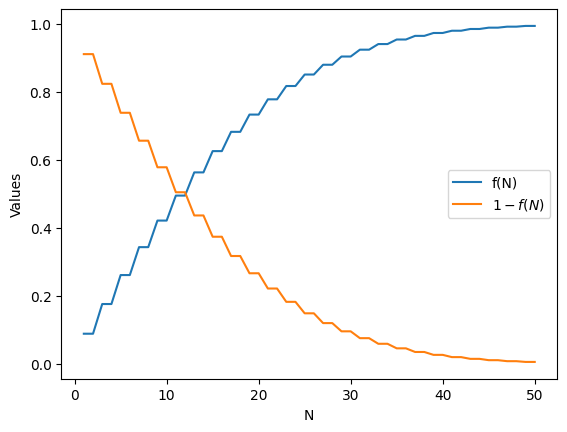
\includegraphics[width=0.5\linewidth]{2-b-iii.png}
\begin{lstlisting}
    For N = 50, f(N) is 0.994534.
\end{lstlisting}
\vspace{0.2cm}
\item[] \textbf{Part III} Based on Part II, we can observe numerically that f(N) approaches to 1 as the N became bigger. The $\mathrm{lim}_{N \rightarrow \infty} f(N) = 1$ indicates that the wave packet can be completely described as a superposition over all the stationary states of the particle-in-a-box. This means that the total probability of finding the particle in any of the box's eigenstates is 1.
\vspace{0.2cm}
\item[] \textbf{Part IV} The function $f(N)$ indicates how many energy eigenstates are required to accurately represent the wave packet. When $f(N)$ is close to 1 for some finite $N$, it means that only the first $N$ terms are needed to approximate the wave packet accurately. 1-$f(N)$ corresponds to some `error' of our approximation. To reach some small `error' that is allowed, we can take some large enough but finite N.\\
\vspace{0.2cm}
\item[] \textbf{Part V} \\

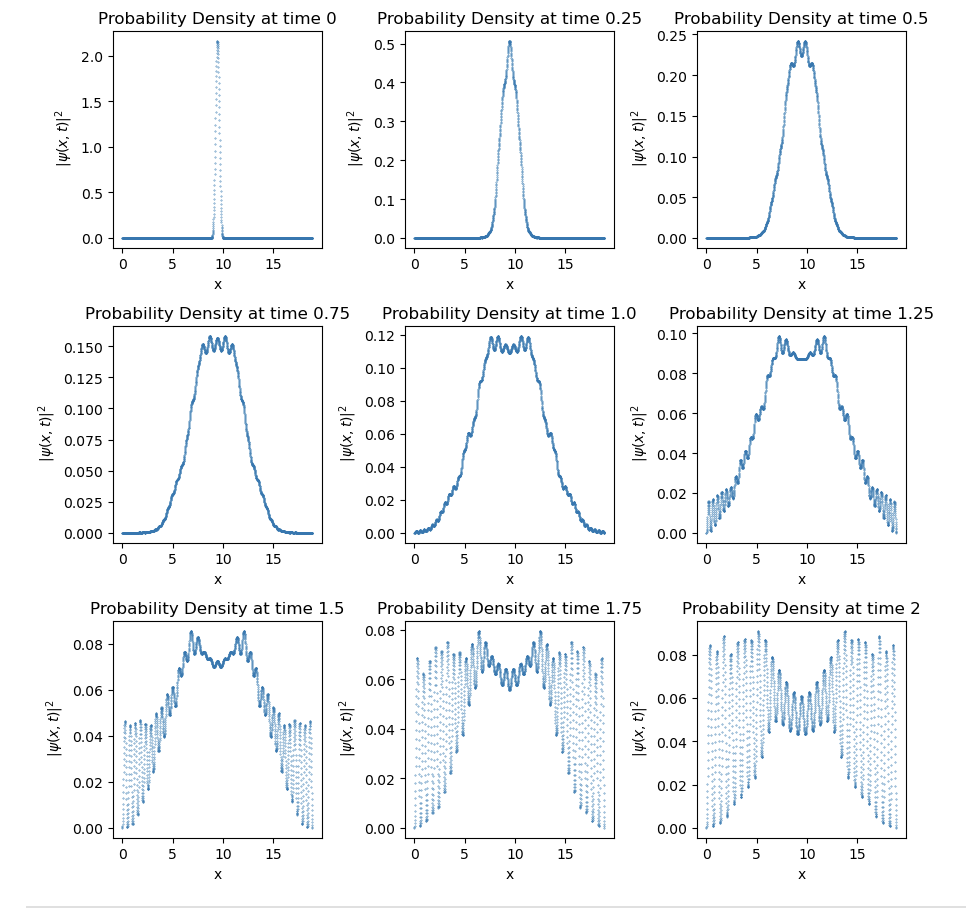
\includegraphics[width=0.6\linewidth]{partVMASTER.png}
\vspace{0.2cm}
\item[] \textbf{Part VI} The plot of $|\Psi(x, t)|^2$ shows how the wave packet spreads and oscillates as time progresses, reflecting the dynamics of a particle in a box. The spreading of the Gaussian wave packet is due to the superposition of multiple energy (momentum) eigenstates, each evolving with its own frequency.
    
\vspace{0.2cm}
\item[] \textbf{Part VII}\\
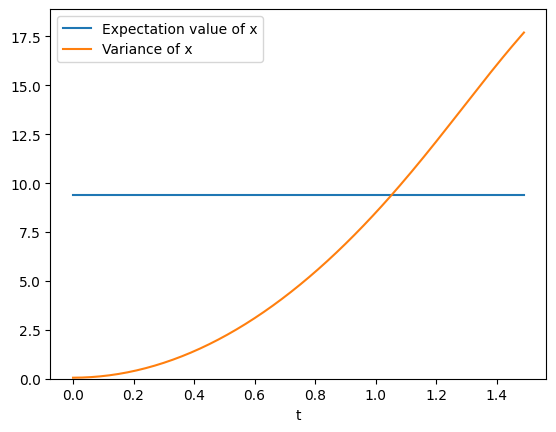
\includegraphics[width=0.5\linewidth]{2-b-vii.png}\\
(we didn't label y-axis, since dimensions of the expectation value and variance are different)

\vspace{0.2cm}
\item[] \textbf{Part VIII} The expectation value $\langle x(t) \rangle$ indicates the average position of the particle as a function of time, while $\langle (x - L/2)^2(t) \rangle$ provides information about the spread of the particle's position around the center of the box, which is dispersion. According to the graph, the probability density is always symmetric about the center of the box and thus the average position of the particle stays in the middle. The time dependence of these quantities reveals the motion and the spreading behavior of the wave packet inside the box.
\end{adjustwidth}



\end{document}
